\label{sec:impacts_inclusive}
\providecommand{\impactswidthscale}{0.6}
%% The \nonprompt photon contribution is estimated using the data-driven approach.
%% The variable considered is $m_{\PZ\PZ\PGg}$.
%% The impacts of the systematic uncertainties on the expected results is shown in Figure \ref{fig:inclusive_cutID_phoCR_mZZGloose}.

\begin{figure}
  \centering
  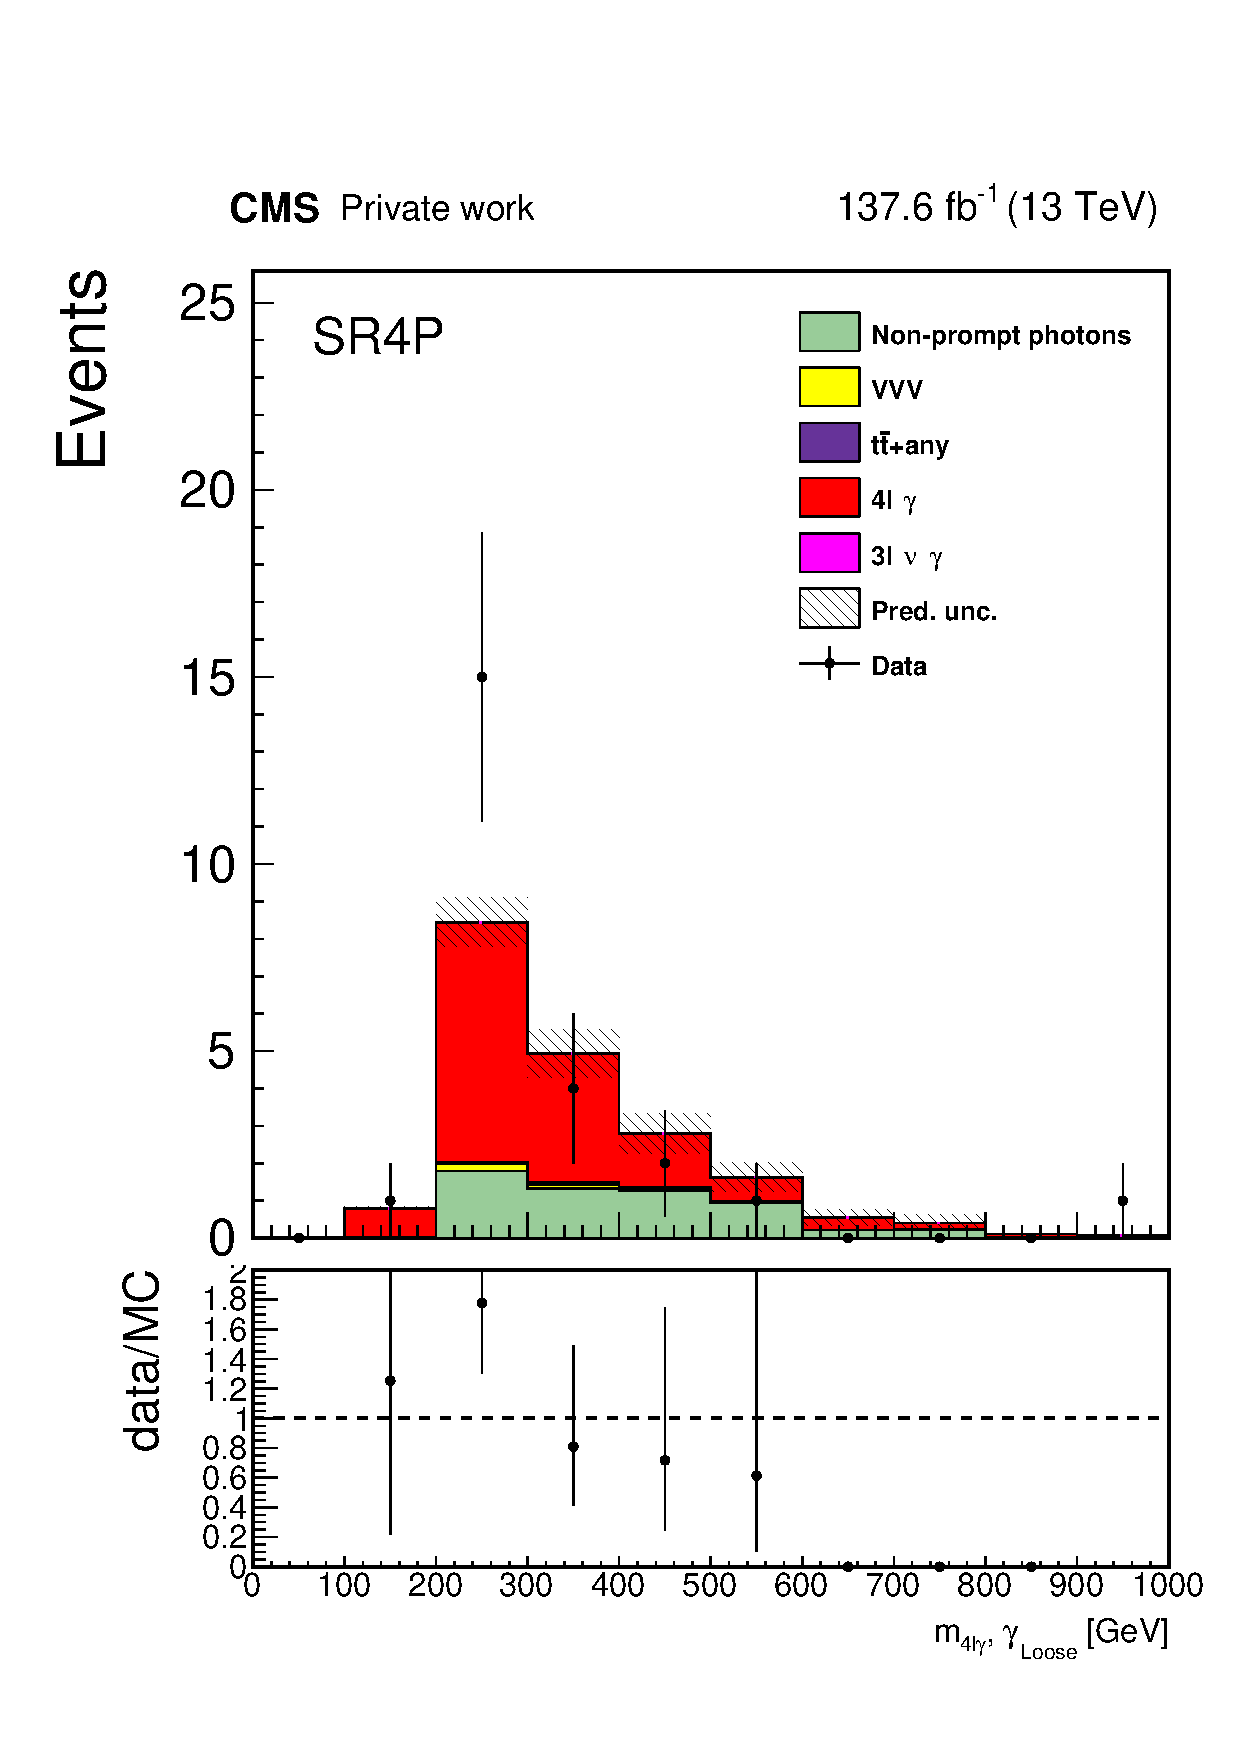
\includegraphics[height=0.33\textheight]{Figures/dataMC/Run2/phoCR/SR4P/SYS_mZZGloose_central_pow.pdf}
  \hfill
  \includegraphics[height=0.33\textheight]{Figures/combine/noPixVeto/Run2_SR4P_phoCR_lepCR_mZZGloose_impacts.pdf}
  \caption{\captionImpact{mass of the $\PZ\PZ\PGg$ system}{Loose}{cut-based ID}{d}{not }}
  \label{fig:inclusive_cutID_phoCR_mZZGloose}
\end{figure}

\begin{figure}
  \centering
  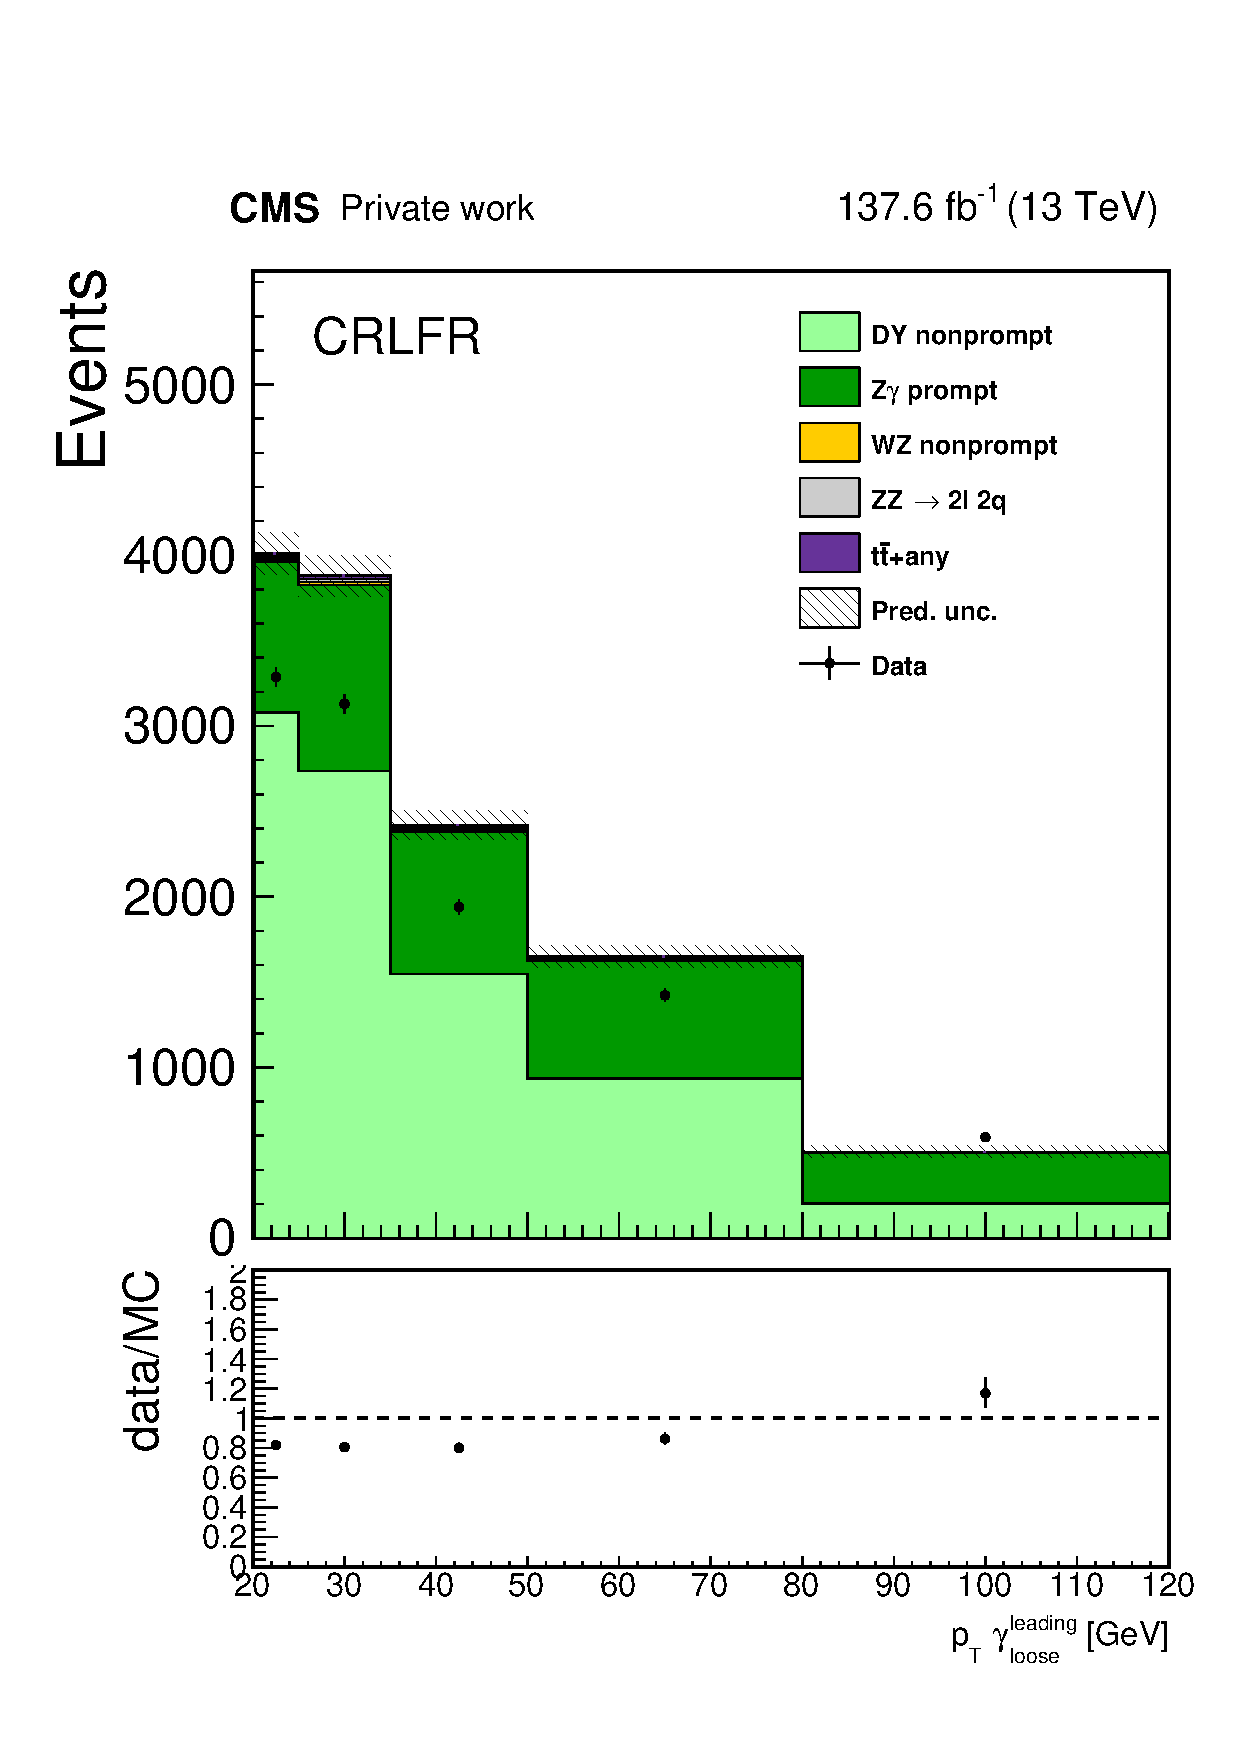
\includegraphics[height=0.33\textheight]{Figures/dataMC/Run2/lepCR/SR4P/lead_loose_pt_pow.pdf}
  \hfill
  \includegraphics[height=0.33\textheight]{Figures/combine/noPixVeto/Run2_SR4P_phoMC_lepCR_loosept_impacts.pdf}
  \caption{\captionImpact{transverse momentum of the photon}{Loose}{cut-based ID}{s}{not }}
  \label{fig:inclusive_cutID_phoMC_loosept}
\end{figure}

\begin{figure}
  \centering
  \includegraphics[height=0.33\textheight]{Figures/dataMC/Run2/lepCR/SR4P/SYS_wp90pt_central_pow.pdf}
  \hfill
  \includegraphics[height=0.33\textheight]{Figures/combine/noPixVeto/Run2_SR4P_phoMC_lepCR_mZZGwp90_impacts.pdf}
  \caption{\captionImpact{mass of the $\PZ\PZ\PGg$ system}{\texttt{wp90}}{MVA ID}{s}{not }}
  \label{fig:inclusive_mvaID_phoMC_mZZGwp90}
\end{figure}

\begin{figure}
  \centering
  \includegraphics[height=0.33\textheight]{Figures/dataMC/Run2/lepCR/SR4P/SYS_wp80pt_central_pow.pdf}
  \hfill
  \includegraphics[height=0.33\textheight]{Figures/combine/noPixVeto/Run2_SR4P_phoMC_lepCR_mZZGwp80_impacts.pdf}
  \caption{\captionImpact{mass of the $\PZ\PZ\PGg$ system}{\texttt{wp80}}{MVA ID}{s}{not }}
  \label{fig:inclusive_mvaID_phoMC_mZZGwp80}
\end{figure}

\begin{figure}
  \centering
  \includegraphics[height=0.33\textheight]{Figures/dataMC/Run2/lepCR/SR4P/SYS_MVAcut_central_pow.pdf}
  \hfill
  \includegraphics[height=0.33\textheight]{Figures/combine/noPixVeto/Run2_SR4P_phoMC_lepCR_MVAcut_impacts.pdf}
  \caption{Distribution and impacts of the systematic uncertainties on the signal strength fit
    on the yield in the various bins of the photon MVA ID.
    \descriptionFakePhoton{s}.
    The FSR cut is not applied.
  }
  \label{fig:inclusive_kin_phoMC_MVAcut}
\end{figure}
